\documentclass{article}
\usepackage[utf8]{inputenc}
\usepackage[margin=1.2in]{geometry}
\usepackage{amsmath, amssymb, amsthm, graphicx, float}
\usepackage{subfig, subfloat}
\allowdisplaybreaks

\begin{document}
\begin{titlepage}
	\centering
	{\LARGE\bfseries Automatic Test generation via Machine Learning \par}
	\vspace{4.5cm}
	{\Large\bfseries Proposal for a design project for the School of Electrical
and Computer Engineering, Cornell University\par}
	\vspace{1.5cm}
	{\large\bfseries By\par}
	\vspace{3cm}
    \flushleft
    {\Large\bfseries Name:~\itshape Arjun Jauhari\par}
	\vspace{0.5cm}
    {\Large\bfseries Project Advisor:~\itshape Prof.~Christoph \textsc{Studer}\par}
	\vspace{0.5cm}
    {\Large\bfseries Signature: \par}
	\vspace{0.5cm}
    {\Large\bfseries Date:~\itshape \today\par}
\end{titlepage}

\section{Abstract}
This project is part of Machine Learning and Education Research aimed to
build an automatic system for generation of test/exams. The project uses 
data dumps from 130+ stack-exchange websites to learn various measures
like difficulty of question, quality of answers, ability of users in a particular 
specialization. The goal is to combine these learned parameters to generate a test on
a particular topic with user defined difficulty. Data on these 130+ stack-exchange
websites is huge, therefore a careful review is required to understand how data 
is arranged, what different attributes mean, so that it can be processed to 
extract out the information of interest. The next phase of the project aims 
to build upon this data a statistical model which will map the interaction
between underlying features of data. The final phase will use this model
to build a full system whose intended application will be to generate a test but
it can be easily extended to applications like ranking users based on their answers,
generating summary of most difficult questions, etc.\\
\section{Introduction}
Recently, use of Internet has become ubiquitous in Education. There is a rapid growth in volume of academic texts available online – lecture excerpts from courses, books chapters, Scholarpedia pages, and sources like technical blogs, Stack Exchange posts, Wikipedia. All these sources available today help a learner(student) to enhance their knowledge without depending much on other human but there are not sufficient ways available to assess one's knowledge in a particular discipline without using an expert(teacher) generated test. 
On the other hand, there is no scarcity of quality questions and corresponding answers on the Internet.
Goal of this project is to use this huge pool of questions and develop 
a novel system which can create tests automatically solving the problem of expert dependent assessment of a learner.\\
\section{Background}
This project aims to use the data available on various Stack Exchange websites to generate tests automatically. But the scope of project is not limited to Stack Exchange only it can easily be extended to other similar websites like Quora.
Stack Exchange provides the dump of their data in a well formatted xml files. Each data dump comprises of 8 files namely -
\begin{itemize}
    \item Badges.xml
    \item \textbf{Comments.xml}
    \item PostHistory.xml
    \item PostLinks.xml
    \item \textbf{Posts.xml}
    \item Tags.xml
    \item \textbf{Users.xml}
    \item Votes.xml
\end{itemize}
Although all of these files contains important information but the one's which are in bold are most relevant for the implementation of this project.
Each line in these files corresponds to a unique Post, User, etc defined by a row tag. All information is stored under attributes of each row. For example a sample row looks like -\\
\\
$<row \textbf{Id}="1" \textbf{PostTypeId}="1" \textbf{CreationDate}="2015-02-03T16:40:26.487" \textbf{Score}="22" \textbf{ViewCount}="307" \textbf{Body}="Sample Question" \textbf{OwnerUserId}="2" \textbf{LastEditorUserId}="2" \textbf{LastEditDate}="2015-02-03T17:51:07.583" \textbf{LastActivityDate}="2015-02-03T21:05:27.990" \textbf{Title}="Sample Title" \textbf{Tags}="line-numbers" \textbf{AnswerCount}="2" \textbf{CommentCount}="0" \textbf{FavoriteCount}="3" />$
\section{Issues}
To generate a test which can be compared to a typical expert generated test,
following issues must be addressed -
\begin{enumerate}
    \item Classify the big pool of questions into various bins of varying difficulty.
        This classification will provide a provision to control the
        overall difficulty level of test.
    \item Quality of each StackExchange user needs to be modeled. How good is a particular user, will
        govern the quality of his contribution which will help in doing \#1 above.
    \item Generated test needs to be diverse i.e. it should have a good mix of
        question's difficulty level, should cover all sub-topics, etc.
    \item Provide multiple choices of answers with a balanced differentiation
        between right and wrong answers. The answers should be such that they
        don't make it obvious for test taker to guess the right one.
    \item Design a metric which can compare the performance of automatic generated
        test with that of expert(teacher) generated test. This is essential to 
        measure the performance of algorithm.
\end{enumerate}
\section{Approach}
To address above mentioned issues a statistical approach is considered 
where first step is to identify the features which are relevant for the model.
Secondly, model needs to learn the parameters which govern the interaction
between these features.
Below I describe the model.
\subsection{Subscripts}
\begin{itemize}
    \item $i$ is subscript for question.
    \item $j$ is subscript for answer.
    \item $k$ is subscript for user.
\end{itemize}
\subsection{Notations}
\begin{enumerate}
    \item $u_k$: Quality measure of the $k$th user.
    \item $q_i$: Quality measure of the $i$th question.
    \item $va_{ij}$: Normalized votes corresponding to $j$th answer of $i$th question. \\
        Calculated as: $va_{ij} = \frac{|sa_{ij}|}{\sum_{j} |sa_{ij}|}$ \\
        where $sa_{ij}$ is the actual votes(score) read from data dump.
    \item $a_{ijk}$: Quality measure of $a_{ij}$th answer given by the $k$th user.
    \item $f_{acc}^{ij}$: Boolean flag telling if this answer was Accepted, read from data dump.
    \item $r_k$: Reputation of the $k$th user, read from data dump.
    \item $N_{a}^{i}$: Number of answer to $i$th question, read from data dump.
    \item $vq_{i}$: Number of votes to $i$th question, read from data dump.
\end{enumerate}

\subsection{Equations}
Below equations model the relation/dependence between
the above defined parameters. \\
\begin{enumerate}
    \item $a_{ijk} = f_a(u_k, q_i, va_{ij}, f_{acc}^{ij})$
    \item $u_k = f_u(\{a_{ijk}\}_{ij}, q_i, r_k)$ , where $\{a_{ijk}\}_{ij}$
        is set of all answers by user k
    \item $q_i = f_q(u_k, N_{a}^{i}, vq_i, \{a_{ijk}\}_{jk})$, where $\{a_{ijk}\}_{jk}$
        is set of all answers to $i$th question
\end{enumerate}
\subsection{Visualization}
\begin{figure}[h]
\centering
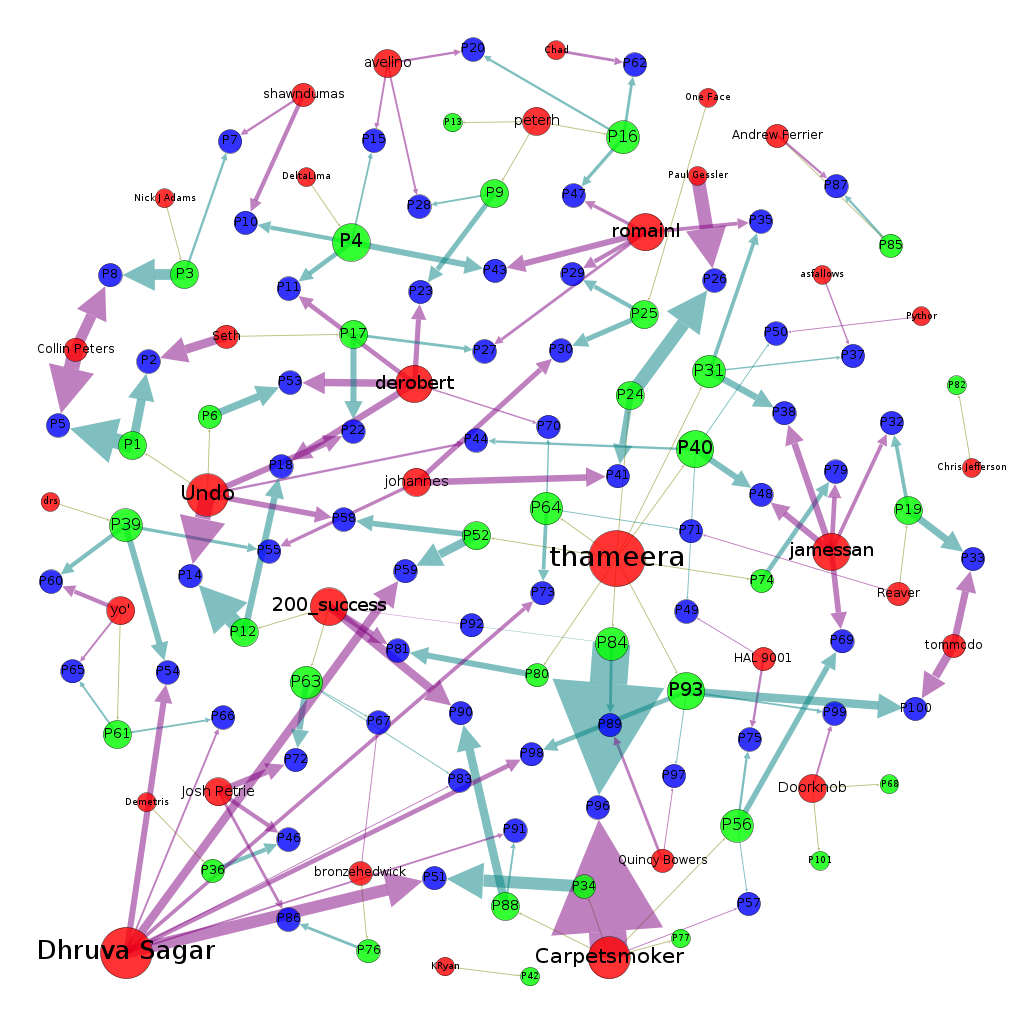
\includegraphics[width=9cm]{proposalimg.png}
\caption{Sample Graph}
\label{fig1:overview}
\end{figure}
To visualise this model I generated graphs using Gephi, figure 1 above
shows one graph on a very small subset of data. Legend for the graph-
\begin{itemize}
    \item Red Nodes: User
    \item Green Nodes: Questions
    \item Blue Nodes: Answers
    \item Green Edge: User2Question(u2q)
    \item Blue Edge: User2Answer(u2b)
    \item Grey Edge: Question2Answer(q2a)
\end{itemize}
The edges connect each user to their post.
Post can be a question(green edge) or an answer(blue edge).
Also, each question is connected to its answers through grey edge.\\
\\
Important details about the graph -
\begin{itemize}
    \item Node size represents, how active is that particular user. For example, user
        with name 'thameera' is the one of the most active user followed by user
        'Dhruv Sagar'.
    \item The thickness of these q2a edges tells the quality of an answer relative to 
all the other answers for same parent question. For example, user 'Carpet Smoker' has
        give one of the best answer.
\end{itemize}

\section{Status}
Currently, the model is very simple with $va_{ij} = \frac{|sa_{ij}|}{\sum_{j} |sa_{ij}|}$, where $sa_{ij}$ is the actual votes(score) read from data dump.\\
and $a_{ijk} = w_1*u_k + w_2*q_i + w_3*va_{ij} + w_4*f_{acc}^{ij}$ \\
\\
As of now weights $w_1, w_2, w_4$ are 0 and $w_3$ is 1, so $a_{ijk} = va_{ij}$ \\
\\
User quality is being modeled as: $u_k \sim \mathcal{N} (mean(\{a_{ijk}\}_{ij}), Var(\{a_{ijk}\}_{ij}))$ \\
\\
Question quality is still not modeled.

\section{Timeline and Deliverables}
\begin{center}
    \begin{tabular}{||l|l|l||}
        \hline
        \textbf{Date} & \textbf{Action Items} & \textbf{Deliverables} \\
        \hline \hline
        October 2015 & 1. Explore Stack Exchange websites  & Summary of findings\\
                     & 2. Understand their data dumps &\\
        \hline
        December 2015 & 1. Extract the relevant features from & Basic implementation of model\\
                      & data and visualize them through graphs & \\
                      & 2. Implement the basic model in python & \\
        \hline
        March 2016 & 1. Extend the model to cover all features & Extended implementation of model \\
                   & 2. Implement Machine Learning algorithm to & \\ 
                   & learn all parameters & \\
        \hline
        May 2016 & 1. Use the learned model to write an algorithm & Final working system\\
                 & which generates automatic test & \\
                 & 2. Evaluate and refine the algorithm & \\
        \hline
    \end{tabular}
\end{center}
\section{Summary}
This project targets to develop a system which automatically generates 
a test using the huge pool of questions and answers available online 
on Stack Exchange websites. Several important issues are being considered. 
I am taking a modular approach and improving incremently to take into account
all the mentioned issues. It is not yet clear how well the above mentioned
model approach will work. Therefore, I am trying to keep the model flexible. So
that it generalize well and can be tweaked easily without much change. 

\end{document}

